\documentclass{article}
\usepackage[utf8]{inputenc}
\usepackage{amsmath}
\usepackage{amsthm}
\usepackage{amsfonts}
\usepackage{graphicx}

\title{Poisson-gamma notes}

\begin{document}
\maketitle

\section{Poisson-gamma dynamical systems}

\begin{figure}[h]
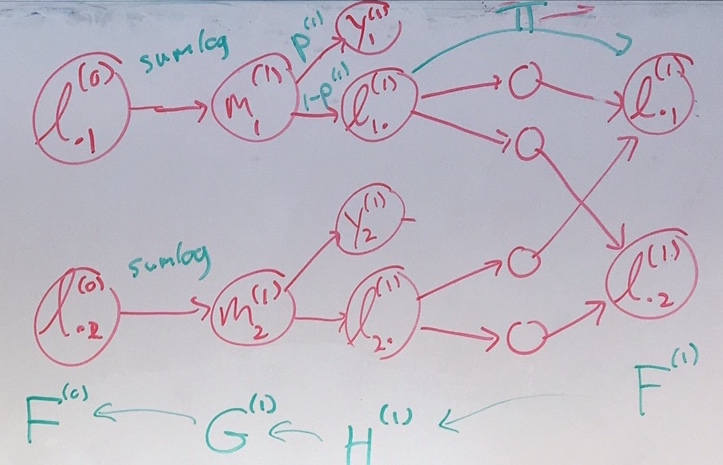
\includegraphics[width=\textwidth]{pgds_cropped}
\end{figure}

Let $F^{(t)}, G^{(t)}, H_y^{(t)}, H_l^{(t)}, g$ be the PGFs of $\mathbf{l.}^{(t)}, \mathbf{m}^{(t)}, \mathbf{y}^{(t)}, (l_{k.}^{(t)})_{k=1}^K, x_{ki}$, respectively. Let $\mathbf{l.}^{(0)}_k \sim Poisson(\lambda_k)$ and $m_k = \sum_i x_{ki} \sim SumLog$.

\begin{align*}
F^{(0)}(\mathbf{s}) &= \sum_{\mathbf{l.}} \prod_k s_k^{l._k} p(\mathbf{s}) \\
&= \prod_k e^{\lambda_k(s_k-1)} \text{, since independent} \\
&= \prod_k s_k^{l._k^{(0)}} \text{, if observed}
\end{align*}

\begin{align*}
G^{(1)}(\mathbf{t}) = F^{(0)}(g(t_1), \ldots, g(t_K))
\end{align*}

\begin{align*}
H^{(1)}(u_1, v_1, u_2, v_2) = G^{(1)}(u_1p + v_1(1-p), u_2p + v_2(1-p))
\end{align*}

\begin{align*}
H_y^{(1)}(u_1, u_2) &= H^{(1)}(u_1, 1, u_2, 1) \\
&= G^{(1)}(u_1p + (1-p), u_2p + (1-p))
\end{align*}

\begin{align*}
H_l^{(1)}(v_1, v_2) &= H^{(1)}(1, v_1, 1, v_2) \\
&= G^{(1)}(p + v_1(1-p), p + v_2(1-p))
\end{align*}

\begin{align*}
F^{(1)}(\mathbf{s}^{(1)}) &= H_l^{(1)}(\mathbf{s}) \\
&= G^{(1)}((1-p)\Pi \mathbf{s}^{(1)} + p \mathbf{1})
\end{align*}

\section{Poisson-gamma belief network}
\begin{figure}[h]
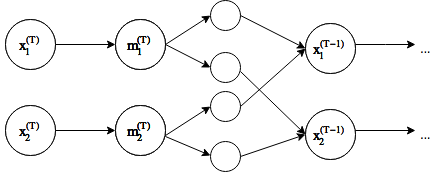
\includegraphics[width=\textwidth]{pgbn}
\end{figure}

Let $K_t$ be the number of hidden units at layer $t$. Define random variables:
\begin{itemize}
\item $\mathbf{x}^{(T)} \sim Pois(-\mathbf{\Phi}^{(T)} \boldsymbol{\theta}^{(T)} \ln (1 - p^{(T)}))$
\item $\mathbf{x}^{(t)} \in \mathbb{Z}^{K_{t-1}}$, where $x_v^{(t)} = \sum_{k=1}^{K_{t-2}} z_{vk}$, for $t = 1, \ldots, T-1$
\item $\mathbf{m}^{(t)}|\mathbf{x}^{(t)} \sim SumLog(\mathbf{x}^{(t)}, p^{(t+1)})$, where $m_k = \sum_{l=1}^{x_k} n_{kl}$
\item $\mathbf{Z}^{(t)}|\mathbf{m}^{(t)} \sim Mult(\mathbf{m}^{(t)}, {\Phi^{(t)}}^T)$
\end{itemize}
and let $F^{(t)}$, $G^{(t)}$, and $g$ be the PGFs of $\mathbf{x}^{(t)}$, $\mathbf{m}^{(t)}$, and $n_{kl}$, respectively.

\begin{align*}
F^{(T)}(\mathbf{s}^{(T)}) = \prod_k e^{\lambda_k(s_k-1)} \text{, since independent} \\
G^{(T)}(\mathbf{t}^{(T)}) = F^{(T)}(g(t_1^{(T)}), \ldots, g(t_{K_{T-1}}^{(T)})) \\
F^{(T-1)}(\mathbf{s}^{(T-1)}) = G^{(T)}({\Phi^{(T)}}^T \mathbf{s}^{(T-1)})
\end{align*}

\end{document}